
\documentclass[a4paper,11pt]{article}
\usepackage{ifpdf}

\ifpdf
\usepackage[pdftex]{graphicx}
\usepackage[pdftex]{hyperref}
\else
\usepackage{graphicx}
\usepackage{hyperref}
\fi

\usepackage[svgnames]{xcolor}
\usepackage{minted}
\usepackage{amsmath}
\usepackage{amssymb}
\usepackage{xspace}
\usepackage{booktabs}
\usepackage{longtable}
\usepackage[top=3cm, bottom=3cm, left=2.5cm,right=2.5cm]{geometry}
%\usepackage[left=3cm,right=3cm]{geometry}

\pagestyle{headings}

\author{Stuart Moodie}
\date{Aug 6, 2013}
\title{Proposed changes for PharmML 0.2.0: Part 2}

\colorlet{bkgd}{gray!5}
%\usemintedstyle{trac}

%\newminted{xml}{bgcolor=bkgd,fontsize=\footnotesize%
%,fontfamily=courier%
%}

\newminted{xml}{fontsize=\footnotesize,fontfamily=courier}

% \newcommand{\inputxml}[1]{\inputminted[bgcolor=bkgd,fontsize=\scriptsize%
% ,fontfamily=courier%
% ]{xml}{codesnippets/#1}}

\newcommand{\cellml}{CellML\xspace}
\newcommand{\sbml}{SBML\xspace}
\newcommand{\sedml}{SED-ML\xspace}
\newcommand{\mathml}{MathML\xspace}
\newcommand{\uncertml}{UncertML\xspace}
\newcommand{\pharmml}{PharmML\xspace}
\newcommand{\xelem}[1]{\texttt{<#1>}\index{XML Element!\texttt{<#1>}}}
\newcommand{\xatt}[1]{\texttt{#1}\index{XML Attribute!\texttt{#1}}}

\begin{document}

\maketitle

\tableofcontents

\section{Introduction}

Following on from the previous proposed changes for version 0.2 of the
\pharmml specification, I have an additional set of proposed
changes. These are either modifications based on feedback from the
first proposal or address new areas not considered in the previous proposal.

% \begin{itemize}
% \item revised parameter model
% \item revised error model
% \item init conditions for derivatives
% \item vector support
% \item new approach to defining a trial
% \item new approach to defining estimation.
% \item defining a simulation where multiple epochs.
% \item drop SBML imports.
% \end{itemize}

\section{Improved Parameter Model}

In the previous proposal I outlined a change to the definition of the
parameter model. The change was to remove assumptions from the
parameter definition and thus to allow parameter definitions that were
not permitted in version 0.1 of the specification. Feedback about this
was generally positive, except Mark Lavielle who felt that this
definition was  a step backwards because we lots the description of
the components of the parameter definition. His proposal was to
define the parameter using one of the following forms:

\begin{align*}
\intertext{Type 1. (implicit) equation type of parameter model}
\psi_i &= H(\beta, c_i, \eta_i)
\intertext{Type 2. Gaussian model with general covariate model}
h(\psi_i) &= H(\beta, c_i) + \eta_i
\intertext{Type 3. Gaussian model with linear covariate model}
h(\psi_i) &= h(\psi_{pop}) + \beta c_i + \eta_i
\end{align*}
with:
\begin{itemize}
\item individual parameter, $\psi_i$
\item population parameter, $\psi_{\textit{pop}}$
\item random effect, $\eta_i$
\item fixed effects, $\beta$
\item arbitrary function , $H$
\item function which transforms the model on both sides, $h$
\end{itemize}

Using these definitions form 3 corresponded to the parameter
definition used in version 0.1\footnote{Well in fact that's almost
  correct. On closer description we found that in version 0.1 we did not explicitly
  constrain ,$h$, the transformation, to be the same on both sides of
  the equation.} and form 1 to the form described in the
previous proposal. Therefore I have updated the parameter definition
to incorporate the three forms above. This should provide total
flexibility, but also make it possible for tools that care to use the
most structures parameter definitions (forms 2 and 3).

As a consequence of the this, the Parameter definition has become more
complicated as we also permit simple parameters definitions, which may
or may not be initialised as well as the individual parameters
definitions above. Therefore in this proposal I have split these
representations between \xelem{SimpleParameter} and
\xelem{IndividualParameter} elements.

Below are some examples:

\subsection{Type 1: Implicit definition}

This might be thought of as the typical way a parameter is defined in NONMEM.

\begin{align*}
V_i &= \mathrm{pop}_{V} \left(\frac{W_{i}}{70}\right)^{\beta_{V}} e^{\left(\eta_{V_i} \right)}
\end{align*}
%
and this can now be encoded, without transformation, as:
%
\begin{xmlcode}
<SimpleParameter symbId="pop_V"/>
<SimpleParameter symbId="omega_V"/>
<SimpleParameter symbId="beta_V"/>
<RandomVariable symbId="eta_V">
    <ct:VariabilityReference>
        <ct:SymbRef block="model" symbId="indiv"/>
    </ct:VariabilityReference>
    <NormalDistribution xmlns="http://www.uncertml.org/3.0" definition="">
        <mean><rVal>0</rVal></mean>
        <stddev><var varId="omega_V"/></stddev>
     </NormalDistribution>                            
 </RandomVariable>
<IndividualParameter symbId="V">
    <ct:Assign>
        <Equation xmlns="http://www.pharmml.org/2013/03/Maths">
            <Binop op="times">
                <ct:SymbRef symbId="pop_V"/>
                <Binop op="times">
                    <Binop op="pow">
                        <Binop op=''divide''>
                            <ct:SymbRef block="c1" symbId="W"/>
                            <ct:Real>70</ct:Real>
                        </Binop>
                        <ct:SymbRef symbId="beta_V"/>
                    </Binop>
                    <Uniop op="exp">
                        <Var symbId="eta_V"/>
                    </Uniop>
                </Binop>
            </Binop>
        </Equation>
    </ct:Assign>
</IndividualParameter>
\end{xmlcode}

Note that this version uses the prototype of \uncertml 3.0.

\subsection{Type 2: Gaussian Model with General Covariate Model}

The following is modified from the NONMEM User Manual\footnote{NONMEM
  Users Guide - Part V: Introductory Guide, p 34.}  and describes an
individual parameter with a non-linear covariate model as follows:
%
\begin{align*}
\mathrm{CL} &= W \left(\Theta_1 -
  \left(\frac{\Theta_2 \mathrm{Cpss_2}}{\Theta_3 +
      \mathrm{Cpss}_2}\right)\right) + \eta_{\mathrm{CL}}
\end{align*}
%
We can express this using the general covariate form of the parameter model as follows: 
%
\begin{xmlcode}
<IndividualParameter symbId="CL">
    <GaussianModel>
        <GeneralCovariate>
            <Assign xmlns="http://www.pharmml.org/2013/03/CommonTypes">
                <Equation xmlns="http://www.pharmml.org/2013/03/Maths"
                    writtenVersion="0.1">
                    <Binop op="times">
                        <Var block="c1" symbId="W"/>
                        <Binop op="minus">
                            <Var symbId="theta1"/>
                            <Binop op="divide">
                                <Binop op="times">
                                    <Var symbId="theta2"/>
                                    <Var symbId="Cpss2"/>
                                </Binop>
                                <Binop op="plus">
                                    <Var symbId="theta3"/>
                                    <Var symbId="Cpss2"/>
                                </Binop>
                            </Binop>
                        </Binop>
                    </Binop>
                </Equation>
            </Assign>
        </GeneralCovariate>
        <RandomEffects>
            <ct:SymbRef symbId="eta_CL"/>
        </RandomEffects>
    </GaussianModel>
</IndividualParameter>
\end{xmlcode}


\subsection{Type 3: Gaussian Model with Linear Covariate}

This is the form familiar from version 0.1 or the \pharmml specification:
%
\begin{align}
\log(V_i) &= \log(\mathrm{pop_{V}}) + \beta_{1,V}\log(W_i/70) + \eta_{V,i}
\end{align}
%
We define this in XML by defining the fixed effect parameters, the random
variable and then the parameter which incorporates these elements into
the above equation.
%
\begin{xmlcode}
<SimpleParameter symbId="beta_V"/>
<SimpleParameter symbId="pop_V"/>
<SimpleParameter symbId="omega_V"/>
<RandomVariable symbId="eta_V">
    <ct:VariabilityReference>
       <ct:SymbRef block="model" symbId="level"/>
    </ct:VariabilityReference>
    <NormalDistribution xmlns="http://www.uncertml.org/3.0" definition="">
        <mean><rVal>0</rVal></mean>
        <stddev><var varId="omega_V"/></stddev>
    </NormalDistribution>                            
</RandomVariable>
<IndividualParameter symbId="V">
    <GaussianModel>
        <Transformation>log</Transformation>
        <LinearCovariate>
            <PopulationParameter>
                <ct:Assign>
                    <ct:SymbRef symbId="pop_V"></ct:SymbRef>
                </ct:Assign>
            </PopulationParameter>
            <Covariate>
                <ct:SymbRef block="c1" symbId="W"></ct:SymbRef>
                <FixedEffect>
                    <ct:SymbRef symbId="beta_V"></ct:SymbRef>
                </FixedEffect>
            </Covariate>
        </LinearCovariate>
        <RandomEffects>
            <ct:SymbRef symbId="eta_V"></ct:SymbRef>
        </RandomEffects>
    </GaussianModel>
</IndividualParameter>
\end{xmlcode}

\subsubsection{The covariate model: incorporating categorical covariates}

A benefit of this approach is that we can revert to dealing with
categorical covariates in the same way as we do in the current version
of the specification, which is clearer and more explicit. So we can
encode:
%
\begin{align*}
1_{\mathrm{ka,TreatSeq}_i=\mathrm{A-B}} &=
\begin{cases}
1 & \text{if } W \text{ has category } \mathrm{A-B}\\
0 & \text{otherwise}
\end{cases}
\intertext{We can incorporate this into the full parameter definition:}
\log(ka_{i}) &= \log(ka_{pop}) + \beta_{ka,TreatSeq}1_{TreatSeq_i=\mathrm{A-B}} + \eta_{ka,i}
\end{align*}
%
as:
%
\begin{xmlcode}
<Parameter symbId="one_ka_treatseq">
    <ct:Symbol>1_ka_treatset</ct:Symbol>
    <ct:Assign>
        <math:Equation writtenVersion="0.1">
            <math:Piecewise>
                <math:Piece>
                    <math:Scalar>1</math:Scalar>
                    <math:Condition writtenVersion="0.1">
                        <math:LogicBinop op="eq">
                            <math:Var block="c1" symbId="W"/>
                            <math:String value="AB"/>
                        </math:LogicBinop>
                    </math:Condition>
                </math:Piece>
                <math:Piece>
                    <math:Scalar>0</math:Scalar>
                    <math:Condition writtenVersion="0.1">
                        <math:Otherwise/>
                    </math:Condition>
                </math:Piece>
            </math:Piecewise>
        </math:Equation>
    </ct:Assign>
</Parameter>
\end{xmlcode}

\subsection{We still retain flexibility}

Just to emphasise the point, all models that were encodable in the
previous proposal are still encodeable. This is the example used in
the previous proposal of an individual parameter definition,
I've taken from Hooker \emph{et al.} 2008\footnote{ Hooker
  et al. ``Population Pharmacokinetic Model for Docetaxel in Patients
  with Varying Degrees of Liver Function: Incorporating Cytochrome
  P450 3A Activity Measurements'' Clinical Pharmacology \& Therapeutics
  84, 111-118 (July 2008) \textbar
  \url{doi:10.1038/sj.clpt.6100476}}. We describe unbound plasma
clearance using the individual parameter $\mathit{CL}_i$ as follows:
%
\begin{align*}
\mathrm{CL}_i &=
\begin{cases}
\eta_{\mathrm{CL}} \cdot \mathrm{CL}_{\mathrm{normal\, LF}} \cdot f_{\mathrm{BSA}} \cdot
f_{\mathrm{AAG}} \cdot f_{\mathrm{ERMBT, normal\, LF}} & \text{if } \mathrm{LFG} = 1\\
\eta_{\mathrm{CL}} \cdot \mathrm{CL}_{\mathrm{impaired\, LF}} \cdot f_{\mathrm{BSA}} \cdot
f_{\mathrm{AAG}} \cdot f_{\mathrm{ERMBT, impaired\, LF}} & \text{if } \mathrm{LFG}
> 1
\end{cases}\\
f_{\mathrm{BSA}} &= \mathrm{BSA} / \overline{\mathrm{BSA}}\\
f_{\mathrm{AAG}} &= 1 + \theta_{\mathrm{AAG-CL}} \cdot \left(\mathrm{AAG} / \overline{\mathrm{AAG}}\right)\\
f_{\mathrm{ERMBT, normal\, LF}} &= 1 + \theta_{\mathrm{ERMBT, normal\, LF}} \cdot
\left(\mathrm{ERMBT} - \overline{\mathrm{ERMBT}}_{\mathrm{normal\, LF}}\right)\\
f_{\mathrm{ERMBT, impaired\, LF}} &= 1 + \theta_{\mathrm{ERMBT, impaired\, LF}} \cdot
\left(\mathrm{ERMBT} - \overline{\mathrm{ERMBT}}_{\mathrm{impaired\, LF}}\right)
\end{align*}
%
With the proposed changes to the paramater model this can be encoded
as follows:
%
\begin{xmlcode}
<SimpleParameter symbId="f_ERMBT_normalLF">
    <ct:Assign>
        <Equation xmlns="http://www.pharmml.org/2013/03/Maths" writtenVersion="0.1">
            <Binop op="plus">
                <Scalar>1</Scalar>
                <Binop op="times">
                    <Var symbId="theta_ERMBT_normalLF"/>
                    <Binop op="minus">
                        <Var symbId="ERMBT"/>
                        <Var symbId="ERMBT_normalLF"/>
                    </Binop>
                </Binop>
            </Binop>
        </Equation>
    </ct:Assign>
</SimpleParameter>
<Parameter symbId="theta_ERMBT_impairedLF"/>
<SimpleParameter symbId="f_ERMBT_impairedLF">
    <ct:Assign>
        <Equation xmlns="http://www.pharmml.org/2013/03/Maths" writtenVersion="0.1">
            <Binop op="plus">
                <Scalar>1</Scalar>
                <Binop op="times">
                    <Var symbId="theta_ERMBT_impairedLF"/>
                    <Binop op="minus">
                        <Var symbId="ERMBT"/>
                        <Var symbId="ERMBT_impairedLF"/>
                    </Binop>
                </Binop>
            </Binop>
        </Equation>
    </ct:Assign>
</SimpleParameter>
<SimpleParameter symbId="theta_AAG_CL"/>
<SimpleParameter symbId="f_AAG">
    <ct:Assign>
        <Equation xmlns="http://www.pharmml.org/2013/03/Maths" writtenVersion="0.1">
            <Binop op="plus">
                <Scalar>1</Scalar>
                <Binop op="times">
                    <Var symbId="theta_AAG_CL"/>
                    <Binop op="minus">
                        <Var symbId="AAG"/>
                        <Var symbId="AAG_bar"/>
                    </Binop>
                </Binop>
            </Binop>
        </Equation>
    </ct:Assign>
</SimpleParameter>
<SimpleParameter symbId="f_BSA">
    <ct:Assign>
        <Equation xmlns="http://www.pharmml.org/2013/03/Maths" writtenVersion="0.1">
            <Binop op="divide">
                <Var symbId="BSA"/>
                <Var symbId="BSA_bar"/>
            </Binop>
        </Equation>
    </ct:Assign>
</SimpleParameter>
<RandomVariable symbId="eta_CL">
    <ct:VariabilityReference>
        <ct:SymbRef symbId="indiv"/>
    </ct:VariabilityReference>
    <Distribution xmlns="http://www.pharmml.org/2013/03/Uncertainty"
    writtenVersion="0.1">
         <!-- Snip -->
    </Distribution>
</RandomVariable>
<IndividualParameter symbId="CL">
    <ct:Assign>
        <Equation xmlns="http://www.pharmml.org/2013/03/Maths" writtenVersion="0.1">
            <Piecewise>
                <Piece>
                    <Binop op="times">
                        <Uniop op="exp"><Var symbId="eta_CL"/></Uniop>
                        <Binop op="times">
                            <Var symbId="CL_normalLDF"/>
                            <Binop op="times">
                                <Var symbId="f_BSA"/>
                                <Binop op="times">
                                    <Var symbId="f_AAG"/>
                                    <Var symbId="f_ERMBT_normalLF"/>
                                </Binop>
                            </Binop>
                        </Binop>
                    </Binop>
                    <Condition writtenVersion="0.1">
                        <LogicBinop op="eq">
                            <Var symbId="LFG"/>
                            <Scalar>1</Scalar>
                        </LogicBinop>
                    </Condition>
                </Piece>
                <Piece>
                    <Binop op="times">
                        <Uniop op="exp">
                            <Var symbId="eta_CL"/>
                        </Uniop>
                        <Binop op="times">
                            <Var symbId="CL_impairedLF"/>
                            <Binop op="times">
                                <Var symbId="f_BSA"/>
                                <Binop op="times">
                                    <Var symbId="f_AAG"/>
                                    <Var symbId="f_ERMBT_impairedLF"/>
                                </Binop>
                            </Binop>
                        </Binop>
                    </Binop>
                    <Condition writtenVersion="0.1">
                        <LogicBinop op="gt">
                            <Var symbId="LFG"/>
                            <Scalar>1</Scalar>
                        </LogicBinop>
                    </Condition>
                </Piece>
            </Piecewise>
        </Equation>
    </ct:Assign>
</individualParameter>
\end{xmlcode}


This example highlights an important question. When is a parameter an
\xelem{IndividualParameter} or a \xelem{SimpleParameter}. If the
equation includes a random variable then you should use the
\xelem{IndividualParameter} element. This is something we could
enforce as a rule within the specification.

\section{Residual Error Model}

In the last proposal we revised the structure of the residual error
model to remove the assumptions ion the definition - as we did with
the parameter model. Unsurprisingly the criticism of the parameter
model changes in the previous proposal also apply to the residual
error model. Therefore I propose to follow the same approach as above
and have a constrained form and a flexible form. What I call the
\emph{Standard} form is set out in equation 52 in Lavielle \emph{et
  al}. There may be other forms that we wish to include buy at the
moment I encode the \emph{Standard} and the implicit form (the latter
name is consistent with that used for the eponymous parameter model).

\begin{align*}
\intertext{Type 1. (implicit) equation type of residual error model}
y_{ij} &= G(x_{ij}, \psi_{i}, \epsilon_{ij})
\intertext{Type 2. Standard residual error model}
u(y_{ij}) &= u(f(x_{ij},\psi_i)) + g(x_{ij}, \psi_i) \epsilon_{ij},
\quad 1 \leq i \leq N, \quad 1 \leq j \leq n_i
\end{align*}
with:
\begin{itemize}
\item N is the number of subjects,
\item $y_i = (y_{ij}, 1 \leq j \leq n_i)$ are the observations for
  individual $i$, with $n_i$, the number of observations of subject
  $i$,
\item $x_i = (x_{ij}, 1 \leq j \leq n_i)$ are regression variables,
\item $\psi_i$, is the vector of individual parameters of subject i, 
\item $u$ is a function which transforms the model on both sides,
\item $\epsilon_{ij}$ is the residual error,
\item $g$ is a function that defines the standard deviation of the
  residual error.
\end{itemize}

Here the XML is modified to permit the definition of residual error
using both these forms. To illustrate this I will show the following
how a residual error model using a combined model described using both forms. 

I should note that the \emph{General} and \emph{Standard} designations
are entirely mine and therefore are probably incorrect. I'd appreciate
advice on how to correctly define the different forms. In the meantime
I will use these terms throughout the rest of the document.

\subsection{General Residual Error Model}

In the first from we define the model as follows:
%
\begin{align*}
C_{o_{ij}} &= C_{s_{ij}} + \left(a + b \cdot f(x_{ij}, \psi_{ij}) \right) \epsilon_{C_{ij}}\\
\intertext{where}
a, b & \text{, are parameters,}\\
C_{o} & \text{, is the output of the observations model,}\\
C_{s} & \text{, is the output of the structural model.}
\end{align*}
%
This can be encoded using the implicit definition as follows:
%
\begin{xmlcode}
<Continuous> <!-- This is C_{o} -->
    <RandomVariable symbId="epsilon_C">
        <VariabilityReference> <!-- This references the variability level -->
            <ct:SymbRef block="obsErr" symbId="residual"/>
        </VariabilityReference>
        <Distribution xmlns="http://www.pharmml.org/2013/03/Uncertainty"
            writtenVersion="0.1">
            <Normal>
              <!-- Snip -->
            </Normal>
        </Distribution>
    </RandomVariable>
    <General  symbId="C">
        <Output>
            <ct:SymbRef block="main" symbId="C"></ct:SymbRef>
        </Output>
        <ct:Assign>
            <!-- C + (combinedErrorModel(a1, b1, C) * epsilon_C) -->
            <math:Equation writtenVersion="0.1">
                <math:Binop op="plus">
                    <math:Var block="main" symbId="C"/> <!-- C_{s} -->
                    <math:Binop op="times">
                        <math:FunctionCall>
                            <math:Var symbId="combinedErrorModel"/>
                            <math:FunctionArgument symbId="a">
                                <math:Var symbId="a1"/>
                            </math:FunctionArgument>
                            <math:FunctionArgument symbId="b">
                                <math:Var symbId="b1"/>
                            </math:FunctionArgument>
                            <math:FunctionArgument symbId="f">
                                <math:Var block="main" symbId="C"/>
                            </math:FunctionArgument>
                        </math:FunctionCall>
                        <math:Var symbId="epsilon_C"/>
                    </math:Binop>
                </math:Binop>
            </math:Equation>
        </ct:Assign>
    </General>
</Continuous>
\end{xmlcode}
%
This is very similar to the previous proposal, but I have introduced
the \xelem{General} element to define the type of error model and this
element now defines observation variable, in this case $C$. I will
explain why this was changed later. Note that multiple \xelem{General}
or \xelem{Standard} elements can be defined within a single
\xelem{Continuous} block. This allows multiple observation variables
to be defined within a single \xelem{Continuous} element.  In this
code snippet you can see that the random variable is defined
explicitly and then used in an equation. As with the parameter
proposal above, this provides maximum flexibility and make the
relationship between the random variable, the error model and the
output variable from the structural model. A validation rule we may
wish to apply is that the equation defining the residual error must
contain references to the random variable defined as a child of the
\xelem{Continuous} element.

\subsection{Standard Residual Error Model}

Our example standard error model is defined as follows:
%
\begin{align*}
\mathrm{Cc}_{o_{ij}} &= \mathrm{Cc}_{s_{ij}} + g(a_i, b_i, \mathrm{Cc}_{s}) \epsilon_{\mathrm{Cc}_{ij}}\\
\intertext{where}
g(a, b, f) &= a + b f.
\end{align*}
%
This is similar to the structure used in version 0.1 of \pharmml, but
the random variable is defined explicitly, the observation variable is
defined within the \xelem{Standard} element and the output variable,
$\mathrm{Cc_o}$ is defined within the \xelem{Output} element. Also the
error model now does not necessarily need to be defined as a function,
but and be defined as an algebraic equation within the
\xelem{math:Equation} elements (note that in the example below a call
to an equation is used).
%
\begin{xmlcode}
<Continuous>
    <RandomVariable symbId="epsilon_Cc">
        <ct:VariabilityReference>
            <ct:SymbRef block="obsErr" symbId="residual"/>
        </ct:VariabilityReference>
        <NormalDistribution xmlns="http://www.uncertml.org/3.0"
            definition="http://www.uncertml.org/distributions/normal">
            <mean><rVal>0</rVal></mean>
            <stddev><var varId="omega_Cc"/></stddev>
        </NormalDistribution>
    </RandomVariable>
    <Standard symbId="Cc">
        <Output>
            <ct:SymbRef block="main" symbId="Cc"></ct:SymbRef>
        </Output>
        <ErrorModel>
            <ct:Assign>
                <math:Equation>
                    <math:FunctionCall>
                        <ct:SymbRef symbId="combinedErrorModel"/>
                        <math:FunctionArgument symbId="a">
                            <ct:SymbRef symbId="a1"/>
                        </math:FunctionArgument>
                        <math:FunctionArgument symbId="b">
                            <ct:SymbRef symbId="b1"/>
                        </math:FunctionArgument>
                        <math:FunctionArgument symbId="f">
                            <math:Equation>
                                <ct:SymbRef block="main" symbId="Cc"/>
                            </math:Equation>
                        </math:FunctionArgument>
                    </math:FunctionCall>
                </math:Equation>
            </ct:Assign>
        </ErrorModel>
        <ResidualError>
            <ct:SymbRef symbId="epsilon_Cc"/>
        </ResidualError>
    </Standard>
</Continuous>
\end{xmlcode}

\subsection{Replicates and Correlation}

Two new features not available in version 0.1 of \pharmml are the
definition of replicate observations and correlation between residual
errors. The former is easy to define. I have just added an
optional \xelem{Replicate} element to the \xelem{general} or
\xelem{Standard} elements that defines the number of replicates to
generate. If not provided then the number of replicates is assumed to
be 1. The XML snippet below shows how we define that $\mathrm{Cc}_o$
has 3 replicates.

\begin{xmlcode}
 <Standard symbId="Cc">
     <Replicates><ct:Int>3</ct:Int></Replicates>
     <Output>
         <ct:SymbRef block="main" symbId="Cc"></ct:SymbRef>
     </Output>
     <ErrorModel>
\end{xmlcode}

To correlate residual errors we simply reuse the constructs for
correlation of random variables in the parameter model. This very
simply allows us to implicitly define a covariance or correlation matrix for
the residual errors in the model. Below is a hypothetical example that
illustrates how it works.

\begin{xmlcode}
            <Continuous>
                <RandomVariable symbId="epsilon_Cc">
                    <ct:VariabilityReference>
                        <ct:SymbRef block="obsErr" symbId="residual"/>
                    </ct:VariabilityReference>
                    <NormalDistribution xmlns="http://www.uncertml.org/3.0"
                        definition="http://www.uncertml.org/distributions/normal">
                        <mean><rVal>0</rVal></mean>
                        <stddev><var varId="omega_Cc"/></stddev>
                    </NormalDistribution>
                </RandomVariable>
                <Standard symbId="Cc">
                    <Replicates><ct:Int>1</ct:Int></Replicates>
                    <Output>
                        <ct:SymbRef block="main" symbId="Cc"></ct:SymbRef>
                    </Output>
                    <ErrorModel>
                        <ct:Assign>
                            <math:Equation>
                                <math:FunctionCall>
                                    <ct:SymbRef symbId="combinedErrorModel"/>
                                    <math:FunctionArgument symbId="a">
                                        <ct:SymbRef symbId="a1"/>
                                    </math:FunctionArgument>
                                    <math:FunctionArgument symbId="b">
                                        <ct:SymbRef symbId="b1"/>
                                    </math:FunctionArgument>
                                    <math:FunctionArgument symbId="f">
                                        <math:Equation>
                                            <ct:SymbRef block="main" symbId="Cc"/>
                                        </math:Equation>
                                    </math:FunctionArgument>
                                </math:FunctionCall>
                            </math:Equation>
                        </ct:Assign>
                    </ErrorModel>
                    <ResidualError>
                        <ct:SymbRef symbId="epsilon_Cc"/>
                    </ResidualError>
                </Standard>
            </Continuous>
            <Continuous>
                <RandomVariable symbId="epsilon_E">
                    <ct:VariabilityReference>
                        <ct:SymbRef block="obsErr" symbId="residual"/>
                    </ct:VariabilityReference>
                    <NormalDistribution xmlns="http://www.uncertml.org/3.0"
                        definition="http://www.uncertml.org/distributions/normal">
                        <mean><rVal>0</rVal></mean>
                        <stddev><var varId="omega_E"/></stddev>
                    </NormalDistribution>
                </RandomVariable>
                <General symbId="E">
                    <ct:Assign>
                        <math:Equation>
                            <math:Binop op="plus">
                                <ct:SymbRef block="main" symbId="E"/>
                                <math:Binop op="times">
                                    <math:FunctionCall>
                                        <ct:SymbRef symbId="constantErrorModel"/>
                                        <math:FunctionArgument symbId="a">
                                            <ct:SymbRef symbId="a2"/>
                                        </math:FunctionArgument>
                                    </math:FunctionCall>
                                    <ct:SymbRef symbId="epsilon_E"/>
                                </math:Binop>
                            </math:Binop>
                        </math:Equation>
                    </ct:Assign>
                </General>
                <Correlation>
                    <ct:VariabilityReference>
                        <ct:SymbRef block="obsErr" symbId="residual"/>
                    </ct:VariabilityReference>
                    <RandomVariable1>
                        <ct:SymbRef symbId="epsilon_C"></ct:SymbRef>
                    </RandomVariable1>
                    <RandomVariable2>
                        <ct:SymbRef symbId="epsilon_E"></ct:SymbRef>
                    </RandomVariable2>
                    <Covariance>
                        <ct:SymbRef symbId="g_C_E">
                    </ct:SymbRef></Covariance>
                </Correlation>
            </Continuous>
\end{xmlcode}

% \section{Support for vectors}

% By vector I mean a one-dimensional array of values or variables of the
% same type. Currently in \pharmml only scalar variable types are
% supported although it is possible to define a vector a literal type
% using the \xelem{Vector} and \xelem{Sequence} elements. The
% realisation that we needed vector support came when I tried to encode
% a first order, linear elimination model with multiple doses. The model
% is as follows:
% %
% \begin{align}
% C(t) &= \sum{i=1}{n} \frac{D_i}{V} \frac{k_a}{k_a-k} \left(
%   e^{-k\left(t-t_{d_i}\right)} -
%   e^{-k_a\left(t-t_{d_i}\right)}\right)
% \label{eqn:multi-dose}
% \end{align}

% I realised that there was no construct for $\Sigma$ in \pharmml and
% that the variables $D$ and $t_D$ were in fact vectors. Obvious really
% but this type of model hadn't been explicitly encoded in \pharmml
% before so we had missed it. This has three important implications:
% \begin{enumerate}
% \item The
% first is that it should be possible to define variables with vector
% type.
% \item \pharmml maths must have operations to support vector indexing
% and operators such as $\Sigma$ and $\Pi$.
% \item Elements in the trial design model must implicitly define vector
%   types. For example the \xelem{DosingTimes}, the definition of Dose
%   Amount, or the variable used to defined a set of individuals in the
%   \xelem{Individual} element.
% \end{enumerate}

% The impact of this is significant. It means that the type system of
% \pharmml will become more complex with a knock on affect on
% validation. I don't think that this can be avoided however. The key
% things it do define it clearly and as simply as possible. It may make
% sense to adopt a type system from another language. Matlab is the
% obvious candidate here, but this may be overkill for what we need.

% The issues that we should seriously think about these:
% \begin{itemize}
% \item Do we only need vector (1D array) support or should we (do we
%   need to) support higher dimension arrays?
% \item How far should we extend vector support in maths? For example
%   should we provide Matlab-like array operators such as \texttt{.*}?
% \item What are the implications for conversion to NONMEM, MONOLIX
%   \emph{et al.}. How do we encode a structural model such as that in
%   equation \ref{eqn:multi-dose} in these target tools?
% \end{itemize}

\section{Fixing the problems in the Trial Design}

\subsection{The problems to be addressed}

In version 0.1 of the specification we provided 2 ways to define the
trial design. You could define the trial structure explicitly using
the \xelem{Design} element and its children or you could define the
trial design in the data file used to describe estimation or
simulation. The first approach has many virtues in that it explicitly
defines what is only implied by the data file approach, it is easy
to understand, non-redundant. The second approach is much less clear
since the dosing regiment, occasion structure, covariates and
objective data are all combined into a single tabular structure that
is inherently very redundant and much harder to understand. However,
the data-file approach is that adopted by tools such as NONMEM and
MONOLIX.

Both approaches, as implemented in the current version of \pharmml,
have limitations that we do need to address in a future release.

{\small%
\begin{longtable}{p{5cm} p{10cm}}\toprule
  \multicolumn{2}{l}{\textbf{Explicit Trial Design}}\\\midrule
  Occasions cannot span epochs. & Because an occasion is a child of an
  \xelem{TrialEpoch} element, it was not designed to span an epoch. It
  is desirable to do this however, so this needs hierarchy relationship
  needs to be re-examined.\\
  Higher levels of variability cannot be represent. & If one wants to
  represent variability between study centres, or countries and one
  wants to represent this variability as a random effect (and not use
  occasions) then \pharmml cannot do this currently.\\
  Washout and run-in periods are treated as epochs. & For consistency we
  should treat these as epochs and so enable occasions to span them.\\
  Varying bolus doses not supported. & It is not possible to define a
  dose amount that changes at each dosing time within a single Bolus
  dosing regimen. It would seem sensible to enable this.\\
  Per-individual doses not supported. & It is not possible to define a
  dose amount that changes per individual. If a dosing amount is
  per-body weight then this can be done in an equation, but you cannot
  currently specify a different absolute dose amount per subject.\\\\
  \multicolumn{2}{l}{\textbf{Design in Data-File}}\\\midrule
  Reading a data-file requires is imperative. & One of the main
  principles of \pharmml is that is declarative. However, the components
  in the estimation and simulation steps that define how a data file is
  read are inherently not. In particular the order that the line of the file
  is read in is significant. In some more complex trial designs there
  may be two or three lines describing the same time-point. Altering the
  order of these lines may, in pathological cases,  alter the result of
  the model.\\
  Easy to generate, difficult to convert to a target. & The current
  data-file structures in the estimation and simulation steps can be
  relatively generated from formats such as NMTRAN and MLXTRAN. However,
  there may be information loss because the \pharmml representation does
  not make any assumptions about the content of the data-file and so
  has to do more work.\\
  Some dosing regimens cannot be described. &  Some dosing regimens
  described in NONMEM cannot be handled by this approach. For example
  a repeated steady state infusion will have values in the
  columns TIME, DOSE, RATE, SS and II, which in combination have
  special meanings. In the current version it is not possible to use this information in the
  datafile to describe such a dosing regiment.\\
Typing of file contents. & Many of the values in a data file are
assigned to variables or parameters in the model. This means that they
should have types that match the element in the model. At present this
is undefined behaviour and the implication is that the item in the
file which be converted from a string to the appropriate
value. However, although this can be validated it is more work and as
with all implicit conversions there may cases where the conversion
made is incorrect. For example 'T' can be a string or a Boolean value for TRUE?\\
Defining possible values. & In come cases, such as defining the set of
individuals, or the possible categorical values for a categorical
covariate such information must be implied by the unique set of values
in the data file. This does not permit one to define categories in
your model, that are not used by the current population of
subjects. It is also potentially error prone. For example in a data
file you may have a set of 10 rows containing the same ID value. What
if the 5th row contains a different value? Is this a mistake or
intended? It's probably a mistake, but when using the contents to
describe the set of all possible values this kind of error cannot be
identified with certainty.\\
\bottomrule
\end{longtable}%
}
A final issue with the approach take in the current specification is
that we have 2 ways of doing the same thing, namely defining the trial
design. Which version should we recommend you use? Worse, they don't
have completely equivalent functionality. The issues associated with
maintaining two ways to do the same thing can be summarised as:
\begin{itemize}
\item It increases the complexity of the language making it harder to
  learn and to validate in software.
\item It increases the effort required to design and test the
  language and to bug fix. Naively, one would expect duplicate structures within the
  language to require double such effort.
\item Duplication also increases the work of converters because they
  now need to map two sets of \pharmml structures to the same target structures.
\item Ironically increased flexibility can make \pharmml harder to
  learn and be detrimental to adoption. Users are unclear which
  structures to use and would tend to want to avoid having to learn
  two ways to do the same thing.
\pharmml. 
\end{itemize}
%
So to conclude, I am advocating that whether we adopt my proposed
changes here, I would recommend that we stick with only one way of
defining the trial design in the next version of \pharmml.

\subsection{Outline of changes to the trial design}

From the critique above, it is inevitable that any changes I am
proposing must also affect the estimation and simulation step sections
of \pharmml. That is the case. In looking at the problem, it occurred
to me that the data-file conflates three classes of information:
\begin{description}
\item[Population] The attributes of the individuals in the study: the
  population in the population model. Each individual has a weight,
  an age, a gender and numerous other properties that may or may not
  be modelled as covariates in a given model. In addition, these
  properties may change over time.
\item[Dosing] When and how a drug or drugs are administered to the
  individuals in the trial.
\item[Measurements] These are the observations taken from each
  individual and specific times during the study. Such measurements
  provide the objective data used during parameter estimation and are
  typically the outputs calculated during a simulation.
\end{description}
Fortunately, I was not alone in this view and the developers of PharML\footnote{I'm not
  sure what the definitive reference of link is to the PharML spec
  is.} had this insight and developed this language accordingly.

By separating out these classes of information you can see that the
information we need to define the clinical trial is as follows:
\begin{description}
\item[Trial Structure] The organisation of the trial, how the subjects
  are grouped into different treatment groups and what the dosing
  regiment is within these treatment groups.
\item[Population] As above, the properties specific to the individual,
  including those that vary over time.
\item[Individual Dosing] This is related to the treatment regimens
  described in the trial structure, but describes the dosing of each
  subject in the study.
\end{description}

In essence my proposal is that we redesign the Design section of
\pharmml to handle the represent the information and that this is the
only place the trial design is defined in \pharmml. That way the
estimation step can be significantly simplified and it's main focus
can be the mapping of the objective data to the model and the
description of an estimation task.

\subsection{Proposed changes}

The first thing to note is that the \xelem{Design} element has been
renamed to \xelem{TrialDesign}. I think this is more consistent with
what we tend to call the information represented in this element. The
next things is the element \xelem{Structure}. This element is used to
define the structure of the trial. To do this I have reused, almost
verbatim, the CDISC Study Design Model\footnote{CDISC URL to go
  here.}, which is an XML representation of a clinical trial. Using
this design gives us the reassurance that we should be able to
represent all trial structures that we are likely to encounter.

The figure below (figure \ref{fig:cdiscstruct}) shows how the CDISC
trial structure is organised. It has five main components:
\begin{description}
\item[Epoch] The epoch defines a period of time during the study which
  has a purpose within the study. For example a washout or a treatment
  window. In CDISC Epochs can describe screening or follow-up periods,
  which are out of the scope of \pharmml. An epoch is usually defined
  by a time period.
\item[Arm] The arm represents a path through the study taken by a
  subject. An arm is composed of a study cell for each epoch in the study.
\item[Cell] The study cell describes what is carried out during an
  epoch in a particular arm. There is only one cell per epoch.
\item[Segment] The segment describes a set of planned observations and
  interventions, which may or may not involve treatment. Note that in
  \pharmml our definition is more limited and we only describe
  treatments. A segment can contains one or more activities.
\item[Activity] The activity is an action that is taken in the
  study. Here it is typically a treatment regimen.
\item[StudyEvent] A study event describes the collection of
  information about a particular individual. In CDISC this can be
  information captured during screening or other non-treatment phases
  of the clinical trial. But here we restrict it to capturing
  observations during the treatment. In \pharmml this is how we
  capture occasions.
\end{description}
 
\begin{figure}[htb]
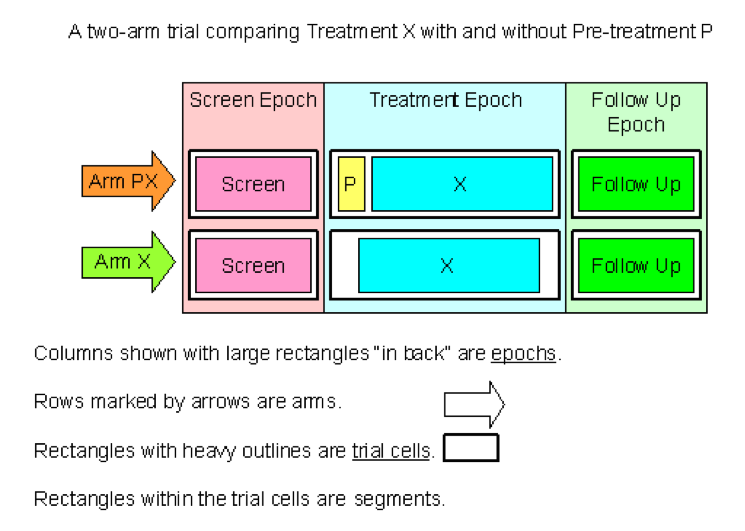
\includegraphics[width=\linewidth]{./CDISCTrialStructure}
\caption{Overview of the Trial Structure used in the CDISC Study
  Design Model.}
\label{fig:cdiscstruct}
\end{figure}


To get an idea how this works in practise, the following example shows
a simple clinical trial describing a steady state model, with one
study arm.

\begin{xmlcode}
    <TrialDesign xmlns="http://www.pharmml.org/2013/03/TrialDesign">
        <Structure>
            <!-- Define the trial structure -->
            <Epoch oid="e1">
                <Order>1</Order>
            </Epoch>
            <Arm oid="a1"/>
            <Cell oid="c1">
                <EpochRef oid="e1"/>
                <ArmRef oid="a1"/>
                <SegmentRef oid="s1"/>
            </Cell>
            <Segment oid="s1">
                <ActivityRef oid="a1"/>
            </Segment>
            <Activity oid="a1">
                <Bolus>
                    <DoseAmount>
                        <DoseVar block="main" symbId="D"/>
                        <ct:Assign>
                            <ct:Real>100</ct:Real>
                        </ct:Assign>
                    </DoseAmount>
                    <SteadyState>
                        <EndTime>
                            <ct:SymbRef symbId="tD"/>
                            <ct:Assign><ct:Real>0</ct:Real></ct:Assign>
                        </EndTime>
                        <Interval>
                            <ct:SymbRef block="p1" symbId="tau"/>
                            <ct:Assign><ct:Real>12</ct:Real></ct:Assign>
                        </Interval>
                    </SteadyState>
                </Bolus>
            </Activity>
        </Structure>
        <Population>
            <!-- Define the variability level associated with the
            population -->
            <ct:VariabilityReference>
                <ct:SymbRef symbId=""></ct:SymbRef>
            </ct:VariabilityReference>
            <!-- Define the individuals -->
            <Individual oid="i">
                <ArmRef oid="a1"/>
                <Replicates>
                    <ct:Int>50</ct:Int>
                </Replicates>
            </Individual>
        </Population>
    </TrialDesign>
\end{xmlcode}

The CDISC like elements are contained in the \xelem{Structure}
tag and you can see how the study is constructed of a single epoch,
with a single arm and a single cell that contains a single
segment. Note, though that this structure is not hierarchical and the
\xelem{Cell} element joins together the arms, epoch and segments
together. Note that a Cell can span several arms contains several
segments. Finally the segment points to an activity the describes
the steady state dosing regimen. The dosing regimen is very similar
to that used in version 0.1 of \pharmml. The details should be ignored
here and please refer to proposed changes to the dosing regimen in the
section below.

Following on from the \xelem{Structure} element is
\xelem{Population}. This is where we describe the individuals in the
study, their attributes (such as weight, gender etc) and assign them
to an arm of the study. In this simple example we only have one arm
and so we assign all the individuals in the study to that arm. As a
shorthand we provide one individual definition and use the element
\xelem{Replicates} to specify how many individuals this
represents. This is obviously useful when simulating a model when (as
in this example) covariates such as weight are calculated for each
individual. An identifier for each individual is created on the fly by
suffixing a sequential number after the identifier. In this case they
would be i1, i2 \ldots i49, i50. While not useful at the moment, such
identifiers will be generated when writing out output to a file. The
\xelem{Replicates} element is optional and later examples will
enumerate the properties of each individual in the population without
using it.

In this simple example the same amount of dose was administered for
each individual. However, in many models the size of the dose varies
per individual. In the example below you can see more complex trial
design with multiple arms and dosing specified per individual. This
corresponds the trial design describing example 6 in the \pharmml
specification. I've reproduced the figure describing it below (figure
\ref{fig:eg6-trial-design}).

\begin{figure}[htb]
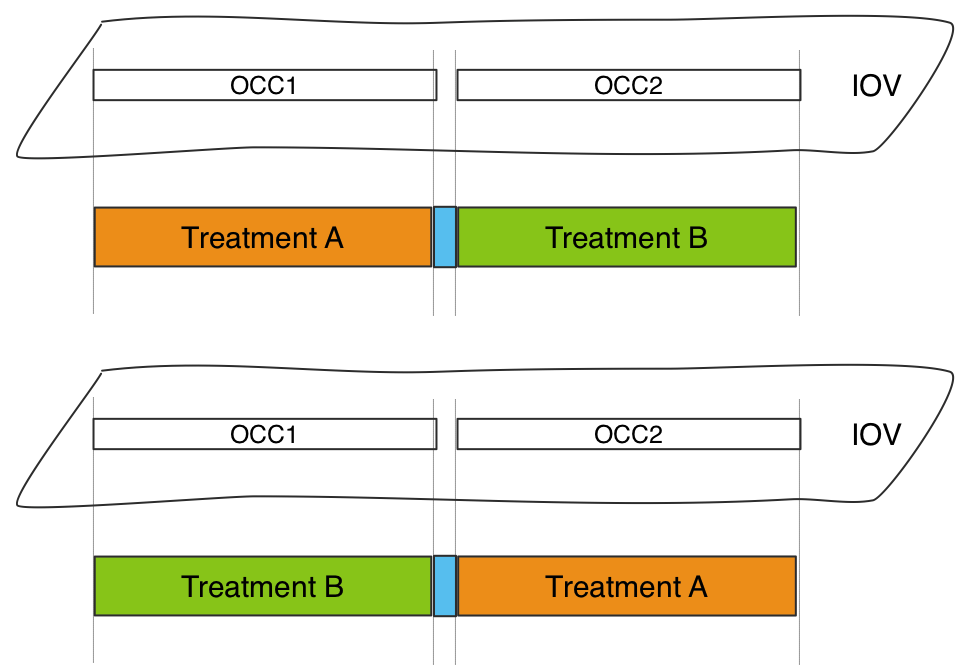
\includegraphics[width=\linewidth]{../pics/iov1simulation_grafio}
\caption{Overview of the trial design used in example 6 of the spec.}
\label{fig:eg6-trial-design}
\end{figure}

\begin{xmlcode}
    <TrialDesign xmlns="http://www.pharmml.org/2013/03/TrialDesign">
        <Structure>
            <Epoch oid="ep1">
                <Order>1</Order>
            </Epoch>
            <Epoch oid="ep2">
                <Order>2</Order>
            </Epoch>
            <Epoch oid="ep3">
                <Order>3</Order>
            </Epoch>
            <Arm oid="a1"/>
            <Arm oid="a2"/>
            <Cell oid="c1">
                <EpochRef oid="e1" />
                <ArmRef oid="a1"/>
                <SegmentRef oid="ta"/>
            </Cell>
            <Cell oid="c2">
                <EpochRef oid="e1" />
                <ArmRef oid="a1"/>
                <SegmentRef oid="tb"/>
            </Cell>
            <Cell oid="c3">
                <EpochRef oid="e2" />
                <ArmRef oid="a1"/>
                <ArmRef oid="a2"/>
                <SegmentRef oid="wash"/>
            </Cell>
            <Cell oid="c4">
                <EpochRef oid="e3"/>
                <ArmRef oid="a1"/>
                <SegmentRef oid="tb"/>
            </Cell>
            <Cell oid="c5">
                <EpochRef oid="e3"/>
                <ArmRef oid="a2"/>
                <SegmentRef oid="ta"/>
            </Cell>
            <Segment oid="ta">
                <ActivityRef oid="d1"/>
            </Segment>
            <Segment oid="tb">
                <ActivityRef oid="d2"/>
            </Segment>
            <Segment oid="wash">
                <ActivityRef oid="w1"/>
            </Segment>
            <Activity oid="d1">
                <Bolus>
                <!-- SNIP -->
                </Bolus>
            </Activity>
            <Activity oid="d2">
                <Bolus>
                <!-- SNIP -->
                </Bolus>
            </Activity>
            <Activity oid="w1">
                <Washout/>
            </Activity>
            <ObservationsEvent oid="occasions">
                <ArmRef oid="a1"/>
                <ArmRef oid="a2"/>
                <ct:VariabilityReference>
                    <ct:SymbRef block="model" symbId="iov"></ct:SymbRef>
                </ct:VariabilityReference>
                <ObservationGroup oid="occ1">
                    <EpochRef oid="ep1"/>
                </ObservationGroup>
                <ObservationGroup oid="occ2">
                    <EpochRef oid="ep3"/>
                </ObservationGroup>
            </ObservationsEvent>
        </Structure>
        <Population>
            <ct:VariabilityReference>
                <ct:SymbRef block="model" symbId="indiv"/>
            </ct:VariabilityReference>
            <Individual oid="i1">
                <ArmRef oid="a1"/>
                <Covariate>
                    <ct:SymbRef block="c1" symbId="Sex"/>
                    <ct:Assign><ct:String>M</ct:String></ct:Assign>
                </Covariate>
                <Covariate>
                    <ct:SymbRef block="c1" symbId="Treat"/>
                    <IVDependent>
                        <EpochRef oid="e1"/>
                        <ct:Assign>
                            <ct:String>A</ct:String>
                        </ct:Assign>
                    </IVDependent>
                    <IVDependent>
                        <EpochRef oid="e3"/>
                        <ct:Assign>
                            <ct:String>B</ct:String>
                        </ct:Assign>
                    </IVDependent>
                </Covariate>
            </Individual>
            <Individual oid="i2">
                <ArmRef oid="a1"/>
                <Covariate>
                    <ct:SymbRef block="c1" symbId="Sex"/>
                    <ct:Assign><ct:String>M</ct:String></ct:Assign>
                </Covariate>
                <Covariate>
                    <ct:SymbRef block="c1" symbId="Treat"/>
                    <IVDependent>
                        <EpochRef oid="e1"/>
                        <ct:Assign>
                            <ct:String>A</ct:String>
                        </ct:Assign>
                    </IVDependent>
                    <IVDependent>
                        <EpochRef oid="e3"/>
                        <ct:Assign>
                            <ct:String>B</ct:String>
                        </ct:Assign>
                    </IVDependent>
                </Covariate>
            </Individual>
            <Individual oid="i3">
                <!-- Omitted the remaining individual definitions
                for brevity -->
            </Individual>
        </Population>
    </TrialDesign>
\end{xmlcode}

In the above example you can see that the more complex trial design
structure is encoded, hopefully as you would expect. Note that the
washout is now defined clearly as an epoch. The new feature that was
not shown in the previous example is the definition of the
occasion as an ObservationsEvent. As you can see this enables us to
define a set of observations, and map them to a variability level. The
duration of each observation (specified by the
\xelem{ObservationGroup} element) can be defined as the duration of a
specified epoch (as in this example) or can be a time period. The
later only makes sense if the epochs define time periods
too\footnote{Note that if each epoch specifies a time period then an
  ObservationEvent can specify a time period that spans multiple
  epochs.}. The \xelem{ObservationsEvent} is associated with an arm,
which means that different sets of inter-occasion variability can be
applied to different arms. I'm not sure if this makes sense or whether
the \xelem{ObservationsEvent} should apply to all arm at the same time
--- and therefore all subjects in the study.

Note also that the definition of the population is richer, with
covariates being defined with each individual. In this example too
each individual in the study is being explicitly defined. Take
particular note of the \xelem{IVDependent} element which is a child of
the \xelem{Individual} element. This is how we define covariates that
are dependent on the independent variable (typically time). In this
example we specify a value for the covariate to be used during a given
epoch. However, it is also possible to specify a time-point
which specifies from which time in the study the covariate value applies.


Perhaps the most complex example is from the Chan and Holford
model\footnote{ref} that defines the most complex trial design
structure that we have so far encoded. It was only possible to encode
this using the data-file approach in the previous version of \pharmml
and even then we had to fix a problem where this method could not
define steady state dosing. As it stands this model cannot be encoded
in version 0.1 of \pharmml. The example is below:

\begin{xmlcode}
    <TrialDesign xmlns="http://www.pharmml.org/2013/03/TrialDesign">
        <Structure>
            <Epoch oid="m0">
                <Start>
                    <ct:Real>0</ct:Real>
                </Start>
                <End>
                    <ct:Real>90</ct:Real>
                </End>
                <Order>1</Order>
            </Epoch>
            <Epoch oid="m6">
                <Start>
                    <ct:Real>408</ct:Real>
                </Start>
                <End>
                    <ct:Real>499</ct:Real>
                </End>
                <Order>2</Order>
            </Epoch>
            <Epoch oid="m12">
                <Start>
                    <ct:Real>908</ct:Real>
                </Start>
                <End>
                    <ct:Real>9999</ct:Real>
                </End>
                <Order>3</Order>
            </Epoch>
            <Epoch oid="m24">
                <Start>
                    <ct:Real>1908</ct:Real>
                </Start>
                <End>
                    <ct:Real>1999</ct:Real>
                </End>
                <Order>4</Order>
            </Epoch>
            <Epoch oid="m48">
                <Start>
                    <ct:Real>3908</ct:Real>
                </Start>
                <End>
                    <ct:Real>3999</ct:Real>
                </End>
                <Order>5</Order>
            </Epoch>
            <Arm oid="a1"/>
            <Cell oid="c1">
                <EpochRef oid="m1"/>
                <ArmRef oid="a1"/>
                <SegmentRef oid="s1"/>
            </Cell>
            <Cell oid="c2">
                <EpochRef oid="m6"/>
                <ArmRef oid="a1"/>
                <SegmentRef oid="s2"/>
            </Cell>
            <Cell oid="c2">
                <EpochRef oid="m12"/>
                <ArmRef oid="a1"/>
                <SegmentRef oid="s2"/>
            </Cell>
            <Cell oid="c2">
                <EpochRef oid="m24"/>
                <ArmRef oid="a1"/>
                <SegmentRef oid="s2"/>
            </Cell>
            <Cell oid="c2">
                <EpochRef oid="m48"/>
                <ArmRef oid="a1"/>
                <SegmentRef oid="s2"/>
            </Cell>
            <Segment oid="s1">
                <ActivityRef oid="exoinf"/>
            </Segment>
            <Segment oid="s2">
                <ActivityRef oid="exoinf"/>
                <ActivityRef oid="oralss"/>
            </Segment>
            <Activity oid="exoinf">
                <Infusion>
                    <DoseAmount>
                        <TargetVar block="sm1" symbId="Ac"/>
                    </DoseAmount>
                    <DosingTimes>
                        <ct:Assign>
                            <ct:Vector>
                                <ct:Real>0</ct:Real>
                                <ct:Real>72</ct:Real>
                            </ct:Vector>
                        </ct:Assign>
                    </DosingTimes>
                    <Duration><ct:SymbRef block="pm1" symbId="TTK0"></ct:SymbRef></Duration>
                </Infusion>
            </Activity>
            <Activity oid="oralss">
                <Infusion>
                    <DoseAmount>
                        <TargetVar block="sm1" symbId="Ac"/>
                        <ct:Assign><ct:SymbRef block="pm1" symbId="Css"/></ct:Assign>
                    </DoseAmount>
                    <SteadyState>
                        <EndTime>
                            <ct:Assign>
                                <ct:Real>0</ct:Real>
                            </ct:Assign>
                        </EndTime>
                    </SteadyState>
                    <Rate><ct:SymbRef block="sm1" symbId="R1"></ct:SymbRef></Rate>
                </Infusion>
            </Activity>
            <ObservationsEvent oid="occ">
                <ArmRef oid="a1"/>
                <ct:Name>Occasions</ct:Name>
                <ct:VariabilityReference>
                    <ct:SymbRef symbId="occ"/>
                </ct:VariabilityReference>
                <ObservationGroup oid="occ1">
                   <Period> <Start>
                        <ct:Real>0</ct:Real>
                    </Start>
                    <End>
                        <ct:Real>24</ct:Real>
                    </End></Period>
                </ObservationGroup>
                <ObservationGroup oid="occ2">
                    <Period><Start>
                        <ct:Real>72</ct:Real>
                    </Start>
                    <End>
                        <ct:Real>90</ct:Real>
                    </End></Period>
                </ObservationGroup>
                <ObservationGroup oid="occ3">
                    <Period><Start>
                        <ct:Real>408</ct:Real>
                    </Start>
                    <End>
                        <ct:Real>457</ct:Real>
                    </End></Period>
                </ObservationGroup>
                <ObservationGroup oid="occ4">
                    <Period><Start>
                        <ct:Real>481</ct:Real>
                    </Start>
                    <End>
                        <ct:Real>499</ct:Real>
                    </End></Period>
                </ObservationGroup>
                <ObservationGroup oid="occ5">
                   <Period> <Start>
                        <ct:Real>908</ct:Real>
                    </Start>
                    <End>
                        <ct:Real>957</ct:Real>
                    </End></Period>
                </ObservationGroup>
                <ObservationGroup oid="occ6">
                    <Period><Start>
                        <ct:Real>981</ct:Real>
                    </Start>
                    <End>
                        <ct:Real>999</ct:Real>
                    </End></Period>
                </ObservationGroup>
                <ObservationGroup oid="occ7">
                    <Period><Start>
                        <ct:Real>1908</ct:Real>
                    </Start>
                    <End>
                        <ct:Real>1957</ct:Real>
                    </End></Period>
                </ObservationGroup>
                <ObservationGroup oid="occ8">
                   <Period> <Start>
                        <ct:Real>1981</ct:Real>
                    </Start>
                    <End>
                        <ct:Real>1999</ct:Real>
                    </End></Period>
                </ObservationGroup>
                <ObservationGroup oid="occ9">
                    <Period><Start>
                        <ct:Real>3908</ct:Real>
                    </Start>
                    <End>
                        <ct:Real>3957</ct:Real>
                    </End></Period>
                </ObservationGroup>
                <ObservationGroup oid="occ10">
                    <Period><Start>
                        <ct:Real>3981</ct:Real>
                    </Start>
                    <End>
                        <ct:Real>3999</ct:Real>
                    </End></Period>
                </ObservationGroup>
            </ObservationsEvent>
            <ObservationsEvent oid="trial">
                <ArmRef oid="a1"/>
                <ct:Name>Trials</ct:Name>
                <ct:VariabilityReference>
                    <ct:SymbRef symbId="occ"/>
                </ct:VariabilityReference>
                <ObservationGroup oid="t1">
                    <EpochRef oid="m1"/>
                </ObservationGroup>
                <ObservationGroup oid="t1">
                    <EpochRef oid="m6"/>
                </ObservationGroup>
                <ObservationGroup oid="t1">
                    <EpochRef oid="m12"/>
                </ObservationGroup>
                <ObservationGroup oid="t4">
                    <EpochRef oid="m24"/>
                </ObservationGroup>
                <ObservationGroup oid="t5">
                    <EpochRef oid="m48"/>
                </ObservationGroup>
            </ObservationsEvent>
        </Structure>
        <Population>
            <ct:VariabilityReference>
                <ct:SymbRef symbId=""/>
            </ct:VariabilityReference>
            <Individual oid="i552">
                <ArmRef oid="a1"/>
                <Covariate>
                    <ct:SymbRef block="c1" symbId="W"/>
                    <IVDependent>
                        <EpochRef oid="m1"/>
                        <ct:Assign><ct:Real>73</ct:Real></ct:Assign>
                    </IVDependent>
                    <IVDependent>
                        <EpochRef oid="m6"/>
                        <ct:Assign><ct:Real>70</ct:Real></ct:Assign>
                    </IVDependent>
                    <IVDependent>
                        <EpochRef oid="m12"/>
                        <ct:Assign><ct:Real>73</ct:Real></ct:Assign>
                    </IVDependent>
                    <IVDependent>
                        <EpochRef oid="m24"/>
                        <ct:Assign><ct:Real>71</ct:Real></ct:Assign>
                    </IVDependent>
                    <IVDependent>
                        <EpochRef oid="m48"/>
                        <ct:Assign><ct:Real>69</ct:Real></ct:Assign>
                    </IVDependent>
                </Covariate>
            </Individual>
        </Population>
        <IndividualDosing>
                <ActivityRef oid="inf1"/>
                <Individual columnRef="id"/>
                <DoseAmount columnRef="dose"/>
                <DosingTime columnRef="t"/>
                <DataSet xmlns="http://www.pharmml.org/2013/03/CommonTypes">
                    <Definition>
                        <Column columnNum="1" columnVar="id"/>
                        <Column columnNum="2" columnVar="t"/>
                        <Column columnNum="3" columnVar="dose"/>
                    </Definition>
                    <Row>
                        <String>i552</String><Real>0</Real><Real>740.37</Real>
                        <String>i552</String><Real>72</Real><Real>740.37</Real>
                        <String>i552</String><Real>409</Real><Real>709.94</Real>
                        <String>i552</String><Real>481</Real><Real>709.94</Real>
                        <String>i552</String><Real>909</Real><Real>740.94</Real>
                        <String>i552</String><Real>981</Real><Real>740.94</Real>
                        <String>i552</String><Real>1909</Real><Real>720.08</Real>
                        <String>i552</String><Real>1981</Real><Real>720.08</Real>
                        <String>i552</String><Real>3909</Real><Real>699.8</Real>
                        <String>i552</String><Real>3981</Real><Real>699.8</Real>
                    </Row>
                </DataSet>
        </IndividualDosing>
    </TrialDesign>
\end{xmlcode}

This uses all the components that you have seen in the previous
examples, with the addition of the \xelem{IndividualDosing}
element. Its purpose is to provide per individual dosing information
a given dosing activity (specified by \verb|<ActivityRef oid="inf1"/>|).
Note that in this example the dose varies with time, but of course it
need not do, in which case the time column and \xelem{DosingTime}
record are omitted. Note that the type of each value is specified
explicitly so it is clear whether the value is compatible with the
information it is being mapped to. If we need dosing information for
more than one dosing activity then multiple \xelem{IndividualDosing}
can be defined.

% \section{Revisions to Dosing regimen}

% I still need to work on this, but going through these examples I have
% realised that the way we handle single, multiple, and SS dosing could
% be improved. The definition of SS dosing in particular is problematic
% at present.

\section{Simplifying the Estimation and Simulation Steps}

A by-product of the redesign of the Trial Design structure is that the
estimation and simulation steps can be considerably
simplified. Perhaps the greatest simplification is with the
\xelem{SimulationStep} which can drop the need to specify the design
in a data file. It now just needs to define initial values and specify
what observations to simulate. A by-product of the re-design is that
we also fix one of the unresolved issues in version 0.1 of
\pharmml. It wasn't clear how to simulate only one epoch since it was
possible for each epoch to have the same time period when separated by
a washout. Now however the epochs must specify consecutive time
periods so the simulation can easily be defined to span all the time
periods in all the epochs of the study.

Finally the use of a data-file in the estimation step becomes very
simple. See for example the estimation step of the Holford and Chan
model:

\begin{xmlcode}
<EstimationStep id="estTask1">
    <ObjectiveDataSet>
        <IndividualMapping>
            <ColumnRef oid="id"/>
        </IndividualMapping>
        <VariableMapping>
            <ColumnRef oid="time"/>
            <ct:SymbRef symbId="t"/>
            <Interpolation>
                <Method name="default"/>
            </Interpolation>
        </VariableMapping>
        <VariableMapping>
            <ColumnRef oid="DV"/>
            <ct:SymbRef block="om1" symbId="CP"></ct:SymbRef>
            <Interpolation>
                <Method name="default"/>
            </Interpolation>
        </VariableMapping>
        <ct:DataSet>
            <ct:Definition>
                <ct:Column columnNum="1" columnVar="id"/>
                <ct:Column columnNum="2" columnVar="time"/>
                <ct:Column columnNum="3" columnVar="DV"/>
            </ct:Definition>
            <ct:Row>
                <ct:String>i552</ct:String><ct:Real>0</ct:Real><ct:Real>0</ct:Real>
            </ct:Row>
            <!-- Snip -->
        </ct:DataSet>
    </ObjectiveDataSet>
    <ParametersToEstimate>
      <!-- Snip -->
    </ParametersToEstimate>
    <EstimationOperation opType="estPop"/>
</EstimationStep>
\end{xmlcode}

Here the mapping of the objective data to the model becomes trivial and
this simplicity enables us to focus on issues we neglected when the
\xelem{EstimationStep} was more complicated. You will notice that each
\xelem{VariableMapping} element contains an \xelem{Interpolation}
element. This allows us to specify how the data should be interpolated
during the estimation procedure. The only available method at the
moment is \emph{default} so clearly this needs more work, but the
objective is clear.

\section{For consideration}

Here I've put changes that we may need to make or at least consider,
but for which I don't have a proposed solution.

\subsection{Initial Conditions}

In version 0.1 of the \pharmml specification and in the previous
proposal we are not clear what we mean by the initial condition of a
derivative variable. I personally have taken it to mean the value of
the variable at the earliest time point use in the
model. Alternatively one might assume that it is the value at
$t=0$. We should be more explicit about this. In addition we may want
to extend this definition in \pharmml to allow the specification of
value at a specific time-point, such as $Ac(t=3) = x$. I have no view
on this, but I'd just like use to do the right thing and be clear
about what we mean.

\subsection{Delaying the use of SBML import}

Currently we import structural models defined in SBML into
\pharmml. Over the past few months I have come to the view that this
is hampering our testing and review of \pharmml. In particular by
delegating a key part of the \pharmml definition we are making it
difficult to spot inconsistencies and error. Perhaps even more
important the implementation of validation, consistency checking and
implementation of software support for \pharmml is significantly
complicated by using SBML.

To support this here are some examples where I think the use of
examples with SBML import caused us to miss an issue:

\begin{itemize}
\item Correctly defining dosing inputs to the structural model. In
  Copenhagen our examples didn't do this correctly, but we missed this
  and the meeting missed this until we switched from the examples
  using SBML to ones where the structural model was defined solely in
  \pharmml.
\item Our definition of initial conditions is vague. This is more
  arguable, but certainly if all our examples contained ODEs defined
  in \pharmml I'm sure the question ``what do we mean by an initial
  condition?'' would have been asked sooner.
\item Multiple dosing requires a vector of doses and dosing
  times. Because we haven't encoded many algebraic models in \pharmml
  itself it wasn't obvious that this was required. Again we tended to
  treat the structural model as a black box and define an import to
  SBML. Preventing SBML import would have forced us to define such
  models in \pharmml.
\end{itemize}

The use of SBML also complicates \pharmml validation and
implementation in the following ways:

\begin{itemize}
\item SBML doesn't have an independent variable (time)
  explicitly. This means that import needs a special construct to map
  the independent variable in \pharmml to that in SBML. We don't at
  present have this construct. This is mainly an issue if you use SBML
  to define an algebraic equation rather than ODE.
\item We need to validate that variables in \pharmml have the same
  types as those in SBML. This can be complicates ad SBML uses a
  different approach to \pharmml and for example doesn't explicitly
  define a variable as a derivative and so this has to be worked out.
\item If as it seems here that \pharmml needs to support vectors then
  this will be a problem when using SBML core. Support for arrays is
  coming in the arrays package, but this is an additional complication
  in supporting SBML.
\item When validating \pharmml using libPharmML we will also have to
  validate the SBML component via libSBML. This is a hassle because it
  is not sufficient that a model is valid SBML, it has to be valid
  SBML which can be correctly mapped to the \pharmml document
  importing it. It will also complicate libPharmML more complex
  because validation will require at least one other XML document to
  be examines, but accessing the other document will be the concern of
  libCombineArchive.
\end{itemize}

I'm not advocating that we drop support for SBML, but rather that we
postpone its inclusion until a later version. That way we can ensure
that the \pharmml definition is correct and it will give us the
ability to implement a fully validating version of
libPharmML. Basically I am advocating that we try and simplify
\emph{before} we reintroduce SBML and the necessary interaction with
libSBML. I suspect if we introduce SBML support later then it will be
much easier to do and get right than if we do it now.

\end{document}
